\scanpage{74}
\diagram{\begin{tikzcd}M\arrow[r]&\mathrm{ab}_k\end{tikzcd}}
$M\otimes N$
\diagram{\begin{tikzcd}X\arrow[r]&M\\X\arrow[r]&N\end{tikzcd}}
\diagram{\begin{tikzcd}
&&M\\
X\deleted{\otimes}X\arrow[r]&M\otimes N\arrow[ur]\arrow[dr]&\\
\mathbf X\arrow[u]&&N
\end{tikzcd}}

$M^{\unsure{\flat|b}}$
\[
L\kappa_M(F)=
\]
\diagram{\begin{tikzcd}\underline M\arrow[r]&M^{\unsure{\flat|b}}\end{tikzcd}}
\deleted{$\longleftrightarrow$}
\diagram{\begin{tikzcd}\unsure{1|e}_{A/x}\arrow[r]&x\end{tikzcd}}
\diagram{\begin{tikzcd}A_{/x}\arrow[r]&A\end{tikzcd}}
\[
\deleted{\unsure{e}}\ 1_{\mathrm{Add}(M_{/x})}\longrightarrow k^{(x)}
\]
\[
M^{\unsure{\flat|b}}=\mathcal M\ni F
\]
\diagram{\begin{tikzcd}N\arrow[r,"f"]&\underline M\end{tikzcd}}
a) $f_!$ exact (à g.)

b) \deleted{$f_!(1_N)=F$}\inserted{$1_N$ projectif}

c) $f_!(1_N)=F$

\fbox{\begin{minipage}{8cm}
a) $f_!$ exact ; $\unsure{f_*}$

b) $1_N\in N$

c) $f_!(1_N)=a$
\end{minipage}}
\margin{fidèle,
$\operatorname{Hom}\mathbin{\text{---}}\operatorname{Hom}$\par
\unsure{unité inj.}}
\diagram{\begin{tikzcd}a\arrow[r,bend right=18]&\text{obj. \deleted{projectif} de \inserted{en $M$}}\end{tikzcd}}
\[
f_!f^*a\mathbin{\text{---}}
\]
$\mathbb Z^{(a)}$

$\underline M^{\unsure{\flat|b}}\qquad F$
\[
N=\{F\in\underline M^{\unsure{\flat|b}}\mid a\otimes_k F\in M\}
\]
\[
\deleted{\unsure{\mathbb Z}}\left\{\begin{array}{l}
\delta(a)\simeq a\otimes a\\
\kappa(a)\simeq k
\end{array}\right.
\]
\figure{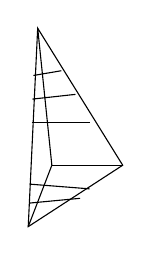
\begin{tikzpicture}[scale=1.2]
\draw(0,0)--(.1,2.1)--(1, .65)--cycle;
\draw(.1,2.1)--(.25,.65)--(0,0);\draw(.25,.65)--(1,.65);
\draw(.055,1.6)--(.35,1.65);\draw(.045,1.35)--(.5,1.4);
\draw(.035,1.1)--(.65,1.1);\draw(.015,.45)--(.65,.4);
\draw(.02,.25)--(.55,.3);
\end{tikzpicture}}
\diagram{\begin{tikzcd}A_{/a}\arrow[r]&A\end{tikzcd}}
\figure{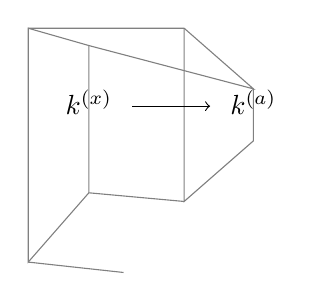
\begin{tikzpicture}[scale=1.1]
\draw[gray](0,0)--(.7,.8)--(.7,2.5)--(0,2.7)--cycle;
\draw[gray](0,2.7)--(1.8,2.7)--(2.6,2)--(.7,2.5);
\draw[gray](1.8,2.7)--(1.8,.7)--(2.6,1.4)--(2.6,2);
\draw[gray](.7,.8)--(1.8,.7);\draw[gray](0,0)--(1.1,-.12);
\node at(.7,1.85){$k^{(x)}$};\node at(2.6,1.85){$k^{(a)}$};
\draw[->](1.2,1.8)--(2.1,1.8);
\end{tikzpicture}}
\diagram{\begin{tikzcd}[column sep=small]
\unsure{x_M,y_M}\arrow[dd,bend right=15]&x&y\arrow[dl,bend left=12]\\
&k^{(x)}&\unsure{k^{(y)}}\\
f_!\underline{\operatorname{Hom}}(x,y)\arrow[r]&\unsure{k^{(\operatorname{Hom}(x,y))}|\operatorname{Hom}(k^{(x)},k^{(y)})}&
\end{tikzcd}}

\rotatebox{-90}{\begin{minipage}{24cm}
\[
K(\mathbb Z,n\qquad\operatorname{Symbin}^*(\qquad L.
\]
\diagram{\begin{tikzcd}[ampersand replacement=\&]
k[t]\arrow[r]\&k\langle t\rangle\\
k\arrow[u]\&
\end{tikzcd}}
\[
k\{P_n(t)\qquad \alpha t\qquad2\alpha
\]
\[
n!\,\unsure{P_n(t)}=t(t-1)\ \inserted{P}\,(t-n+1)
\]
\[
\frac{a(a-1)}{\deleted{\unsure{a}}2}\mathbin{\text{---}}\qquad\frac{t^2}{2}
\]
\[
x(x-1)\mathbin{\text{---}}(x-p+1)\qquad t(t-1)
\]
\[
\frac{x(x-1)}{2}=
\]
\deleted{$\unsure{x(t-1)=\frac{x}{p}}$}
\[
1+at+P(a)t^2
\]
\[
\unsure{1+bt+P(b)}
\]
\[
at+P(a)
\]
\[
(a+b)t+P(a+b)t^2
\]
\[
P(a+b)=P(a)+P(b)+ab
\]
$\mathbb Z\langle t\rangle$\qquad binomial

\figure{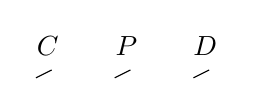
\begin{tikzpicture}
\node at(0,.4){$C$};\node at(1,.4){$P$};\node at(2,.4){$D$};
\draw(-.15,0)--(.05,.1);\draw(.85,0)--(1.05,.1);\draw(1.85,0)--(2.05,.1);
\end{tikzpicture}}
$a(b)$
\end{minipage}}

$\mathbb Z^{(a)}$

\rotatebox{90}{\begin{minipage}{27cm}
\diagram{$\begin{array}{lllllll}
\texttt{PPPPPPPPPPP}&\texttt{RRRRRRRRRRR}&\texttt{EEEEEEEEEEEE}&\texttt{DDDDDDDDD}&\texttt{OOOOOOOOOOOO}&\texttt{NN\ \ \ \ \ \ \ \ NN}&\texttt{TTTTTTTTTTTT}\\
\texttt{PPPPPPPPPPPP}&\texttt{RRRRRRRRRRRR}&\texttt{EEEEEEEEEEEE}&\texttt{DDDDDDDDDD}&\texttt{OOOOOOOOOOOO}&\texttt{NNN\ \ \ \ \ \ \ NN}&\texttt{TTTTTTTTTTTT}\\
\texttt{PP\ \ \ \ \ \ \ \ PP}&\texttt{RR\ \ \ \ \ \ \ \ RR}&\texttt{EE}&\texttt{DD\ \ \ \ \ \ \ DD}&\texttt{OO\ \ \ \ \ \ \ \ OO}&\texttt{NNNN\ \ \ \ \ \ NN}&\texttt{\ \ \ \ \ TT}\\
\texttt{PP\ \ \ \ \ \ \ \ PP}&\texttt{RR\ \ \ \ \ \ \ \ RR}&\texttt{EE}&\texttt{DD\ \ \ \ \ \ \ \ DD}&\texttt{OO\ \ \ \ \ \ \ \ OO}&\texttt{NN\ NN\ \ \ \ \ NN}&\texttt{\ \ \ \ \ TT}\\
\texttt{PP\ \ \ \ \ \ \ \ PP}&\texttt{RR\ \ \ \ \ \ \ \ RR}&\texttt{EE}&\texttt{DD\ \ \ \ \ \ \ \ DD}&\texttt{OO\ \ \ \ \ \ \ \ OO}&\texttt{NN\ \ NN\ \ \ \ NN}&\texttt{\ \ \ \ \ TT}\\
\texttt{PPPPPPPPPPPP}&\texttt{RRRRRRRRRRRR}&\texttt{EEEEEEEE}&\texttt{DD\ \ \ \ \ \ \ \ DD}&\texttt{OO\ \ \ \ \ \ \ \ OO}&\texttt{NN\ \ \ NN\ \ \ NN}&\texttt{\ \ \ \ \ TT}\\
\texttt{PPPPPPPPPPP}&\texttt{RRRRRRRRRRR}&\texttt{EEEEEEEE}&\texttt{DD\ \ \ \ \ \ \ \ DD}&\texttt{OO\ \ \ \ \ \ \ \ OO}&\texttt{NN\ \ \ \ NN\ \ NN}&\texttt{\ \ \ \ \ TT}\\
\texttt{PP}&\texttt{RR\ \ \ \ RR}&\texttt{EE}&\texttt{DD\ \ \ \ \ \ \ \ DD}&\texttt{OO\ \ \ \ \ \ \ \ OO}&\texttt{NN\ \ \ \ \ NN\ NN}&\texttt{\ \ \ \ \ TT}\\
\texttt{PP}&\texttt{RR\ \ \ \ \ RR}&\texttt{EE}&\texttt{DD\ \ \ \ \ \ \ \ DD}&\texttt{OO\ \ \ \ \ \ \ \ OO}&\texttt{NN\ \ \ \ \ \ NNNN}&\texttt{\ \ \ \ \ TT}\\
\texttt{PP}&\texttt{RR\ \ \ \ \ \ RR}&\texttt{EE}&\texttt{DD\ \ \ \ \ \ \ DD}&\texttt{OO\ \ \ \ \ \ \ \ OO}&\texttt{NN\ \ \ \ \ \ \ NNN}&\texttt{\ \ \ \ \ TT}\\
\texttt{PP}&\texttt{RR\ \ \ \ \ \ \ RR}&\texttt{EEEEEEEEEEEE}&\texttt{DDDDDDDDDD}&\texttt{OOOOOOOOOOOO}&\texttt{NN\ \ \ \ \ \ \ \ NN}&\texttt{\ \ \ \ \ TT}\\
\texttt{PP}&\texttt{RR\ \ \ \ \ \ \ \ RR}&\texttt{EEEEEEEEEEEE}&\texttt{DDDDDDDDD}&\texttt{OOOOOOOOOOOO}&\texttt{NN\ \ \ \ \ \ \ \ \ N}&\texttt{\ \ \ \ \ TT}
\end{array}$}
\begin{tabular}{l}
\texttt{****A END JOB 1282 PREDONT - CRAY OUTPUT - ROOM 6.48.16 PM 19 MAY 82 R6.PR1 SYS JES2 JOB 1282 END A****}\\
\texttt{****A END JOB 1282 PREDONT - CRAY OUTPUT - ROOM 6.48.16 PM 19 MAY 82 R6.PR1 SYS JES2 JOB 1282 END A****}\\
\texttt{****A END JOB 1282 PREDONT - CRAY OUTPUT - ROOM 6.48.16 PM 19 MAY 82 R6.PR1 SYS JES2 JOB 1282 END A****}\\
\texttt{****A END JOB 1282 PREDONT - CRAY OUTPUT - ROOM 6.48.16 PM 19 MAY 82 R6.PR1 SYS JES2 JOB 1282 END A****}\\
\texttt{****A END JOB 1282 PREDONT - CRAY OUTPUT - ROOM 6.48.16 PM 19 MAY 82 R6.PR1 SYS JES2 JOB 1282 END A****}\\
\texttt{****A END JOB 1282 PREDONT - CRAY OUTPUT - ROOM 6.48.16 PM 19 MAY 82 R6.PR1 SYS JES2 JOB 1282 END A****}
\end{tabular}
\end{minipage}}
\mspage{73}
